\documentclass[10pt]{article}
\usepackage[paperwidth=11.8cm,paperheight=4.5cm,margin=0pt]{geometry}
\usepackage{tikz}
\usepackage{amsmath,amssymb}
\usepackage{mathptmx}
\pagestyle{empty}
\begin{document}
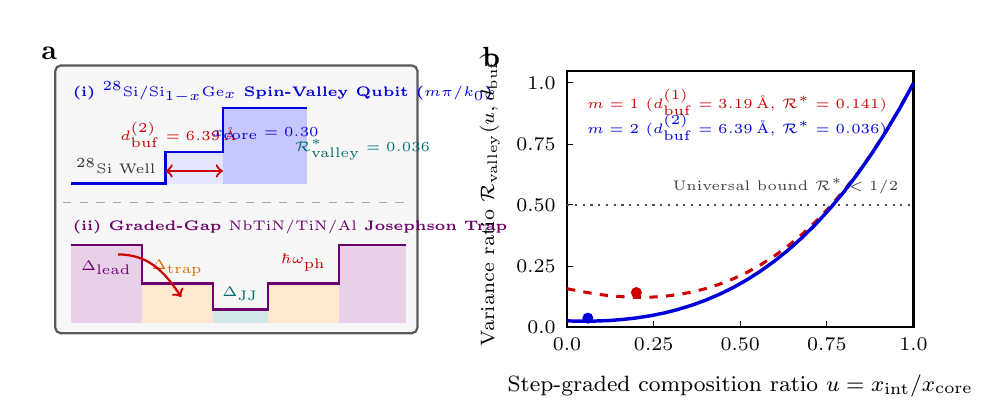
\begin{tikzpicture}[x=1cm,y=1cm]
  \useasboundingbox (0,0) rectangle (11.8,4.5);

  % Panel a: Unified Step-Graded Spin-Valley & Superconducting Qubit Schematic
  \node[anchor=north west,font=\bfseries\normalsize] at (0.05,4.38) {a};
  \draw[thick,rounded corners=2pt,fill=black!3,draw=black!65] (0.35,0.62) rectangle (4.95,4.02);

  % Top sub-panel: Si/SiGe Step-Graded Quantum Well
  \node[anchor=north west,font=\tiny\bfseries,blue!85!black] at (0.45,3.94) {(i) ${}^{28}\mathrm{Si}/\mathrm{Si}_{1-x}\mathrm{Ge}_x$ Spin-Valley Qubit ($m\pi/k_0$)};
  % Step-graded conduction band profile
  \fill[blue!10] (1.75,2.52) rectangle (2.48,2.92);
  \fill[blue!22] (2.48,2.52) rectangle (3.55,3.48);
  \draw[thick,blue!85!black] (0.55,2.52) -- (1.75,2.52) -- (1.75,2.92) -- (2.48,2.92) -- (2.48,3.48) -- (3.55,3.48);
  \draw[<->,red!80!black,thick] (1.75,2.68) -- (2.48,2.68);
  \node[font=\tiny,red!80!black] at (1.92,3.14) {$d_{\mathrm{buf}}^{(2)}=6.39\,\text{\AA}$};
  \node[font=\tiny,black!80] at (1.12,2.74) {${}^{28}\mathrm{Si}$ Well};
  \node[font=\tiny,blue!85!black] at (3.02,3.16) {$x_{\mathrm{core}}=0.30$};
  \node[font=\tiny,teal!85!black] at (4.25,2.95) {$\mathcal{R}_{\mathrm{valley}}^*=0.036$};

  \draw[dashed,black!35] (0.45,2.28) -- (4.85,2.28);

  % Bottom sub-panel: Graded-Gap Superconducting Josephson Junction Trap
  \node[anchor=north west,font=\tiny\bfseries,violet!85!black] at (0.45,2.18) {(ii) Graded-Gap $\mathrm{NbTiN/TiN/Al}$ Josephson Trap};
  \fill[violet!18] (0.55,0.75) rectangle (1.45,1.74);
  \fill[orange!18] (1.45,0.75) rectangle (2.35,1.25);
  \fill[teal!18] (2.35,0.75) rectangle (3.05,0.92);
  \fill[orange!18] (3.05,0.75) rectangle (3.95,1.25);
  \fill[violet!18] (3.95,0.75) rectangle (4.80,1.74);
  \draw[thick,violet!85!black] (0.55,1.74) -- (1.45,1.74) -- (1.45,1.25) -- (2.35,1.25) -- (2.35,0.92) -- (3.05,0.92) -- (3.05,1.25) -- (3.95,1.25) -- (3.95,1.74) -- (4.80,1.74);
  \node[font=\tiny,violet!90!black] at (1.00,1.45) {$\Delta_{\mathrm{lead}}$};
  \node[font=\tiny,orange!85!black] at (1.90,1.45) {$\Delta_{\mathrm{trap}}$};
  \node[font=\tiny,teal!85!black] at (2.70,1.12) {$\Delta_{\mathrm{JJ}}$};
  \draw[->,red!80!black,thick] (1.15,1.62) .. controls (1.55,1.62) and (1.75,1.38) .. (1.95,1.08);
  \node[font=\tiny,red!80!black] at (3.50,1.52) {$\hbar\omega_{\mathrm{ph}}$};

  % Panel b: Universal Step-Graded Disorder Variance Ratio R*(u, d_buf)
  \node[anchor=north west,font=\bfseries\normalsize] at (5.65,4.38) {b};
  \draw[thick] (6.85,0.70) rectangle (11.25,3.95);
  \foreach \v/\y in {0.0/0.70, 0.25/1.47, 0.50/2.25, 0.75/3.02, 1.0/3.80} {
    \draw (6.85,\y) -- (6.93,\y);
    \node[left,font=\scriptsize] at (6.83,\y) {\v};
  }
  \foreach \xval/\xpos in {0.0/6.85, 0.25/7.95, 0.50/9.05, 0.75/10.15, 1.0/11.25} {
    \draw (\xpos,0.70) -- (\xpos,0.78);
    \node[below,font=\scriptsize] at (\xpos,0.68) {\xval};
  }
  \node[below,font=\footnotesize] at (9.05,0.22) {Step-graded composition ratio $u = x_{\mathrm{int}}/x_{\mathrm{core}}$};
  \node[rotate=90,above,font=\scriptsize] at (6.12,2.32) {Variance ratio $\mathcal{R}_{\mathrm{valley}}(u,d_{\mathrm{buf}})$};

  % Universal ceiling R = 0.5 line
  \draw[dotted,black!70,thick] (6.85,2.25) -- (11.25,2.25);
  \node[anchor=south east,font=\tiny,black!75] at (11.18,2.27) {Universal bound $\mathcal{R}^* < 1/2$};

  \draw[red!80!black,dashed,line width=1.1pt] (6.850,1.185) -- (7.026,1.150) -- (7.202,1.120) -- (7.378,1.097) -- (7.554,1.083) -- (7.730,1.075) -- (7.906,1.077) -- (8.082,1.088) -- (8.258,1.110) -- (8.434,1.142) -- (8.610,1.186) -- (8.786,1.242) -- (8.962,1.311) -- (9.138,1.394) -- (9.314,1.492) -- (9.490,1.605) -- (9.666,1.735) -- (9.842,1.882) -- (10.018,2.047) -- (10.194,2.232) -- (10.370,2.436) -- (10.546,2.661) -- (10.722,2.909) -- (10.898,3.180) -- (11.074,3.475) -- (11.250,3.795);
  \draw[blue!85!black,line width=1.25pt] (6.850,0.776) -- (7.026,0.772) -- (7.202,0.774) -- (7.378,0.780) -- (7.554,0.794) -- (7.730,0.814) -- (7.906,0.841) -- (8.082,0.876) -- (8.258,0.921) -- (8.434,0.975) -- (8.610,1.039) -- (8.786,1.114) -- (8.962,1.200) -- (9.138,1.300) -- (9.314,1.413) -- (9.490,1.540) -- (9.666,1.682) -- (9.842,1.840) -- (10.018,2.015) -- (10.194,2.208) -- (10.370,2.420) -- (10.546,2.651) -- (10.722,2.904) -- (10.898,3.177) -- (11.074,3.474) -- (11.250,3.795);

  % Global minima markers
  \fill[red!80!black] (7.730,1.136) circle (2.0pt);
  \fill[blue!85!black] (7.114,0.811) circle (2.0pt);

  \node[anchor=north west,font=\tiny,red!80!black] at (6.98,3.84) {$m=1$ ($d_{\mathrm{buf}}^{(1)}=3.19\,\text{\AA}$, $\mathcal{R}^*=0.141$)};
  \node[anchor=north west,font=\tiny,blue!85!black] at (6.98,3.52) {$m=2$ ($d_{\mathrm{buf}}^{(2)}=6.39\,\text{\AA}$, $\mathcal{R}^*=0.036$)};
\end{tikzpicture}
\end{document}
